\section{Data \& EDA}
\label{sec:data}
For our dataset, we use WikiArt Refined \citep{tan2019wikiart}, which
contains $\sim$81k paintings, each labeled with one of 27 styles
(Figure~\ref{fig:class-distribution}). The dataset has a supplied
70/30 training / validation split which maintains class balance.
Image size and resolution show no outliers. However,
the dataset suffers from an extreme class imbalance, with a
$133.3\times$ imbalance ratio between the extrema classes:
Impressionism (13{,}060) versus the smallest leaves
Analytical\_Cubism (77), Action\_painting (98), and
Synthetic\_Cubism (216). 

\begin{figure}[t]
 \centering
 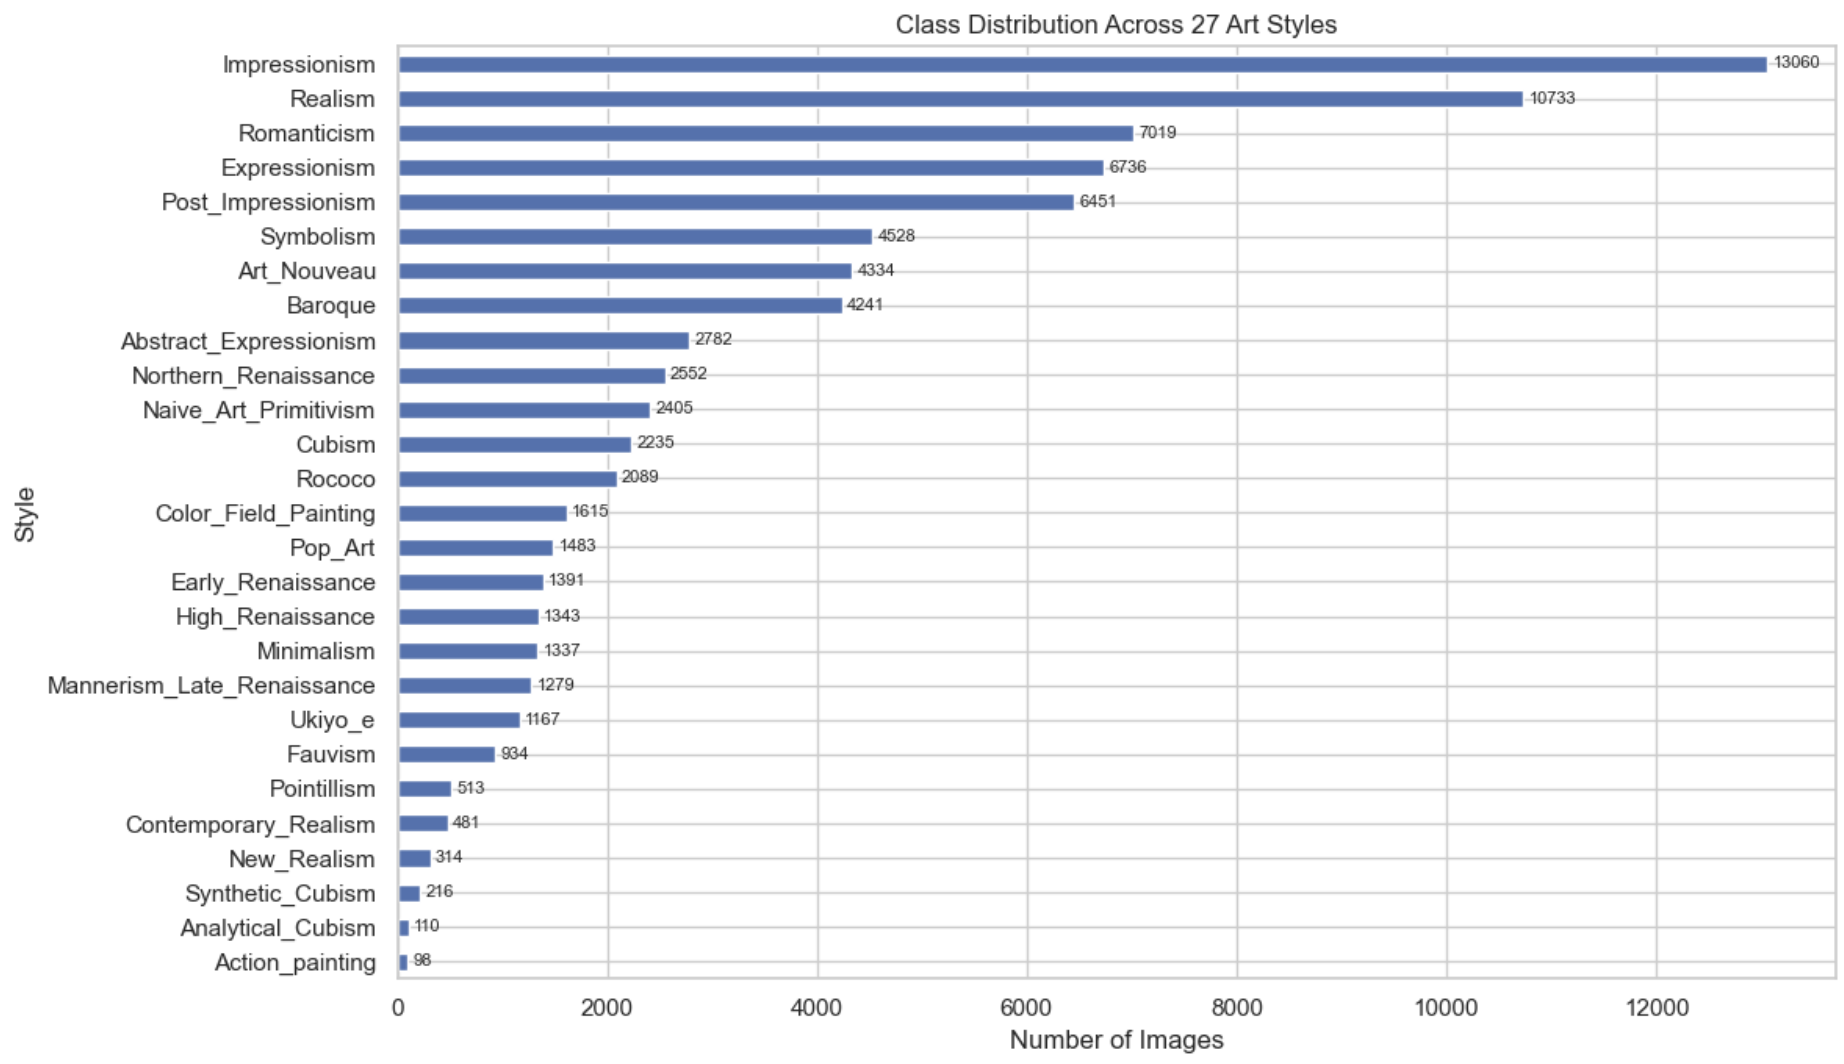
\includegraphics[width=0.85\linewidth]{figures/Class_Distribtuion.png}
 \caption{Per-style image counts on the WikiArt Refined corpus.}
 \label{fig:class-distribution}
\end{figure}

Two design choices follow from this imbalance: we report balanced
accuracy alongside top-1 so the rare leaf styles are not drowned by
Impressionism, and our classification head is a prototype softmax
(Section~\ref{sec:methods}) whose logits depend only on the geometric
distance from each style prototype, with no per-class bias term.

The choice of ground-truth tree is non-unique: WikiArt ships no
hierarchy, and art-history offers several credible taxonomies. Given
the arbitrary nature of this labeling, we evaluate three trees. The
\emph{default} tree (Appendix~\ref{app:tree}) follows the standard
art-historical lineage from Renaissance through Cubism. The
\emph{chronological} tree groups styles into six era buckets
(Renaissance, Baroque--Rococo, 19th century, early 20th century,
modern post-war, non-Western). The \emph{flat} tree makes every style
a direct child of the root and serves as a null whose pairwise
distances are constant off-diagonal. For a tree $T$ with leaves
$u, v$, we define tree distance as the unweighted shortest-path edge
count
\[
 d_T(u, v) = \mathrm{depth}(u) + \mathrm{depth}(v)
           - 2\,\mathrm{depth}\!\bigl(\mathrm{LCA}(u, v)\bigr),
\]
where $\mathrm{LCA}$ is the lowest common ancestor
(Figure~\ref{fig:tree-distance-matrices}). Phase~3 of
Section~\ref{sec:results} re-trains under each tree to test whether
the geometry winner depends on this choice.

\begin{figure}[t]
 \centering
 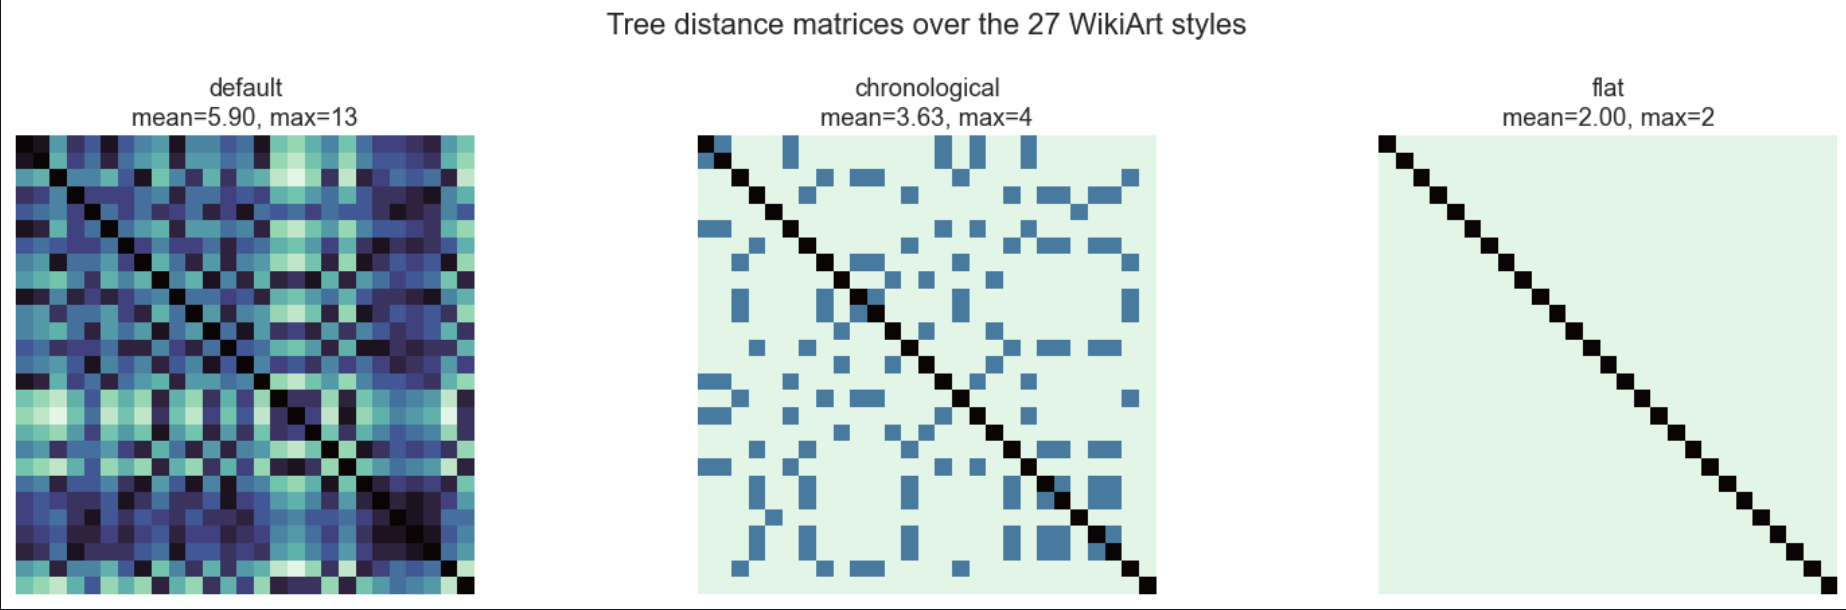
\includegraphics[width=\linewidth]{figures/dist_mat.png}
 \caption{Distance matrices for reference
 hierarchies: default lineage, chronological grouping,
 flat null}
 \label{fig:tree-distance-matrices}
\end{figure}


